\documentclass[]{thesis-ekf}
\usepackage[T1]{fontenc}
\PassOptionsToPackage{defaults=hu-min}{magyar.ldf}
\usepackage[magyar]{babel}
\usepackage{mathtools,amssymb,amsthm,pdfpages}
\footnotestyle{rule=fourth}

\newtheorem{tetel}{Tétel}[chapter]
\theoremstyle{definition}
\newtheorem{definicio}[tetel]{Definíció}
\theoremstyle{remark}
\newtheorem{megjegyzes}[tetel]{Megjegyzés}

\begin{document}

\institute{Matematikai és Informatikai Intézet}
\title{Játékfejlesztés Unity keretrendszerben}
\author{Szabó Márk\\programtervező informatikus Bsc.}
\supervisor{Troll Ede\\tanársegéd}
\city{Eger}
\date{2025}
\maketitle

\tableofcontents

\chapter*{Bevezetés}
\addcontentsline{toc}{chapter}{Bevezetés}

\chapter{Technológiai áttekintés}

Manapság a játékfejlesztés legelterjedtebb módja a játékmotorok használata. Alternatív megoldásként azonban még előfordul az API-alapú fejlesztés is, amely során különféle API-k – például grafikai vagy multimédiakezelő API-k – segítségével történik a fejlesztés. A szakdolgozatom elkészítéséhez én a játékmotor-alapú fejlesztést választottam, így ki tudtam használni az általa kínált lehetőségeket és eszközöket.

\section{Enginek}

A játékmotorok olyan fejlesztői környezetek, amelyek célja, hogy egyszerűsítsék és felgyorsítsák a játékok fejlesztésének folyamatát. Egy tipikus játékmotor különböző komponenseket és funkciókat szolgáltat a fejlesztőnek, mint például: grafikai renderelést, fizikai szimulációt, animációkezelést, hangkezelést. A játékmotorok használata megkönnyíti a fejlesztők dolgát, viszont nem ad annyi rugalmasságot, mint az API alapú fejlesztés. \cite{WikipediaGameEngine}

\subsection{Unreal}

Az Unreal Engine egy professzionális, nagy teljesítményű játékmotor, amelyet az Epic Games fejleszt. Főbb előnyei közé tartozik a kiemelkedő grafikája. Az ingyenes hozzáférése és a vizuális programozást lehetővé tevő Blueprint rendszere miatt kisebb fejlesztők körében is népszerűvé vált. Elsősorban C++-ban történő fejlesztésre optimalizált, de a már említett Blueprint-rendszernek köszönhetően programozói tapasztalat nélkül is lehetséges játékot fejleszteni benne. A játékmotorban sok újrahasználható komponens megtalálható, így a gyakran használt dolgokat pl. karakter mozgást, nem kell felépíteni az alapoktól. A játékmotort 3D játékok fejlesztésére találták ki. \cite{WikipedaiUnreal}

\subsection{Godot}

A Godot egy nyílt forráskódú, ingyenesen elérhető játékmotor. Nagy előnye a könnyű használhatóság, a kis erőforrás igénye, valamint a nyílt forráskód nyújtotta rugalmasság és közösségi támogatás. Támogatja a 2D és 3D játékfejlesztést egyaránt, natív scriptnyelve a GDScript (Pythonhoz hasonló nyelv). \cite{GitHubGodot}

\subsection{Unity}

A Unity az egyik legismertebb és legelterjedtebb játékmotor a piacon, amely támogatja a mobil, asztali, konzolos, valamint webes játékok fejlesztését 2D és 3D játékokhoz egyaránt. Jelentős előnye a könnyen tanulható felhasználói felület és a jól dokumentáltság. Elsősorban a C\# nyelvet használja scriptelésre, de támogatja a vizuális programozást is. A játékmotorhoz tartozik több különböző előfizetési szint is, de van ingyenesen használható verziója is.  Mivel a C\# közel áll hozzám, tapasztalatom is van már ezzel a játékmotorral és maga a játékmotor adottságai pont megfeleltek a szakdolgozatom követelményeihez, ezért erre a játékmotorra esett a választásom. Erről a játékmotorról \aref{ch-unity}. fejezetben bővebben írok. \cite{WikipediaUnity}

\section{Többjátékos technológia a játékfejlesztésben}

A mai megjelenő játékok nagy része már tartalmaz valamiféle többjátékos módot. Ez a játékfejlesztés elején még csak helyi megoldásokat jelentett, de ma már hatalmas online terekben játszódó játékokról is beszélhetünk.

\subsection{Korai megoldások}

Többjátékossal játszható játék először stratégia kör alapú játékokban jelent meg, de ez még nem egyidejű játékot jelentett. Ezek után egyidejű többjátékos játék lehetősége először egy 2 játékossal egyszerre egy helyen játszható játékkal jött létre, ez a játék volt a jól ismert Pong. A Pong után kezdtek egyre jobban elterjedni a helyi többjátékos játékok, ahol az egymás elleni játék helyett, egymással együtt működve is tudtunk játszani. Egy népszerű módszer a helyi többjátékos játékok megvalósításánál az osztott képernyő, ahol általában el van választva a kijelző több egyenlő részre, ahol 1-1 részt 1-1 játékos kezelhet. A 2000-es évek elején pedig már megjelent az online többjátékos játékok lehetősége is, ahol már nem volt szükség egy térben tartózkodni a többi játékossal. \cite{MediumMultiplayer}

\subsection{Kliens-Szerver}

A Kliens-Szerver architektúra az egyik legtöbbet használt módszer az online többjátékos játékok megvalósításához. Az architektúrában 2 szerep van:

\begin{itemize}
	\item Szerver:
	\begin{itemize}
		\item Felelős a játék logikájának feldolgozásáért, az interakciók kezelésért, az erőforrások kezeléséért és a kliensek közötti információk szinkronizálásáért.
		\item A szerver lehet egyetlen gépen elhelyezett (dedikált szerver) vagy a játékosok egyik gépén futó (hosztolt szerver).
		\item A szervernek egyszerre több kliens kéréseit kell kezelnie, ami azt jelenti, hogy skálázhatónak és hatékonynak kell lennie.
	\end{itemize}
	\item Kliens:
	\begin{itemize}
		\item A játékos játékpéldánya. Bemeneti parancsokat küld a szervernek, és frissítéseket kap a játék állapotáról.
		\item Felelősek a játékvilág rendereléséért és a helyi interakciók kezeléséért.
	\end{itemize}
\end{itemize}

\begin{figure}[ht!]
	\centering
	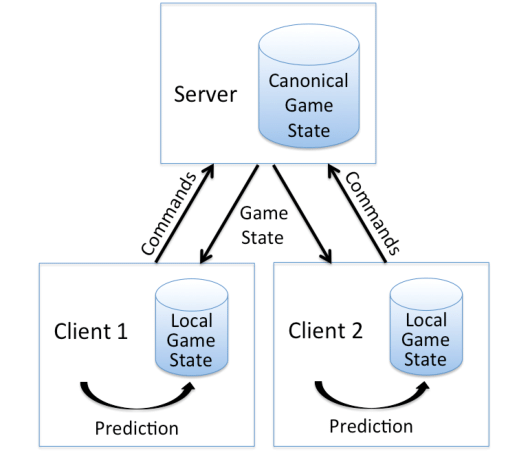
\includegraphics[width=15cm]{ClientServer}
	\caption{Kliens-Szerver architektúra}
	\label{fig-clientserver}
\end{figure}

A kliens és a szerver megbízható hálózati protokoll (pl. TCP vagy UDP) segítségével kommunikál, és olyan csomagokat küld, amelyek a játékosok interakcióiról, játékeseményekről és állapotfrissítésekről tartalmaznak információkat. 
 
Végső sorban szerver ellenőriz minden interakciót és csak ő tud dönteni a változásokról. Ez azért jó, mert így a csalásokkal szemben is védekezik a játék. 

Mivel mindig várni kell a szerver által küldött információra egy interakció esetén, így késleltetés léphet fel, főleg lassabb internet kapcsolat esetén. Erre egy módszer amit alkalmazni szoktak a klienseknél az úgynevezett predikció, ahol a helyi interakció alapján a kliens megpróbálja kitalálni mi fog ténylegesen történni. \cite{MediumClientServer}

\subsection{Peer-to-Peer (P2P)}

A P2P architektúra lényege, hogy a játékosok közvetlen kapcsolatot létesítenek egymással, így nincs szükség központi szerverekre, ellentétben a Kliens-Szerver architektúránál. Ebben a felépítésben, minden játékosnak helyi szinten kezeli a rendszer a játéklogikát.

\begin{figure}[ht!]
	\centering
	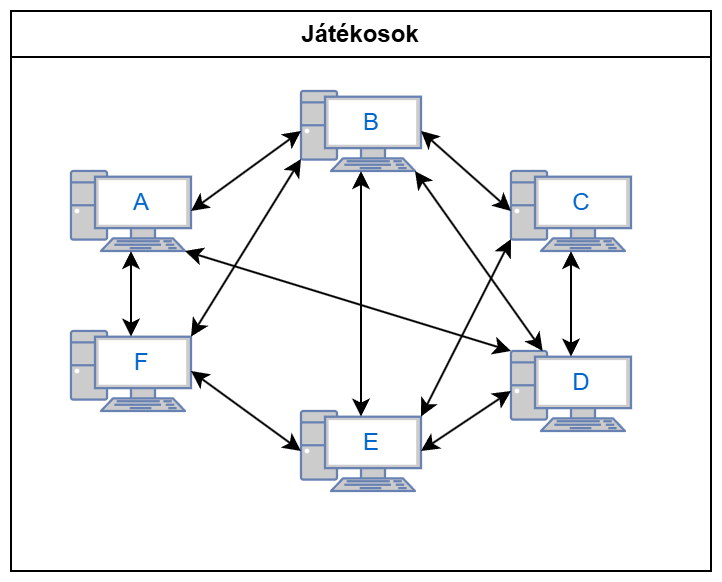
\includegraphics[width=10cm]{P2P}
	\caption{Peer-to-Peer architektúra}
	\label{fig-p2p}
\end{figure}

A P2P architektúra előnyei a Kliens-Szerver architektúrával szemben:
\begin{itemize}
	\item Mivel a játékosok közvetlen kapcsolatot alakítanak ki egymással, így általában gyorsabb a válaszidő.
	\item Sokkal költség hatékonyabb megoldás, mivel nem kell egy központi szerver üzemeltetésére költeni.
\end{itemize}

Mivel ebben a felépítésben nincs egy központi szerver, ami ellenőrző szerepet is tölt be, így a csalások kiszűrése több gondot okozhat. Mint minden felépítésnek, ennek is vannak előnyei és hátrányai is. Ezt az architektúrát kisebb játékos létszám igényű játékoknál célszerű használni. A szakdolgozatom során egy a Unity által létrehozott P2P architektúrán alapuló technológiát alkalmazok, amiről \aref{sec-relay}. szekcióban bővebben írok. \cite{WikipediaP2P} \cite{MediumP2P}

\chapter{Unity}
\label{ch-unity}

\section{Relay}
\label{sec-relay}

\chapter{Rendszerterv}
Azok az elemek, amiket tanultatok RFT-n, azok kerülnek ide

\section{Rendszer célja}
\section{Követelmények}
\section{Architekturális terv}
PC unity, Mobile unity, SharedDLL
\section{Használt fejlesztői eszközök}

\chapter{Saját szoftver megvalósítása}

\section{Texas Hold'Em}

A póker a világ egyik legismertebb kártyajátéka, amelyben a játékosok célja, hogy a saját lapjaikból a lehető legjobb kombinációt kialakítva megszerezzék az asztalon lévő kasszát. A póker számos különböző szabályrendszerrel rendelkező változatban létezik.

A \emph{Texas~Hold’Em} a közösségi pókerjátékok legnépszerűbb formája, amelyet jellemzően 2 és 10 játékos között játszanak. Ez egy viszonylag zárt struktúrájú játék, ahol a licitálás menete állandó szabályok szerint zajlik.

\subsection{Szabályok ismertetése}

Ebben a fejezetben a póker legelterjedtebb, hivatalos versenyeken is alkalmazott szabályrendszere kerül bemutatásra. Ami közös az összes variációban, hogy a játékot 52~lapos francia kártyával játsszák dzsókerek nélkül.

\subsubsection{Játék menete}

A játék során három fontos szerep forog körbe a játékosok között, amit ,,gombokkal'' jelölünk. Ezek a szerepek az osztó, kis vak és nagy vak. Az osztótól balra ülő játékos lesz a kis vak, a kis vaktól balra ülő pedig a nagy vak. Az osztót pedig több különböző módon választhatjuk meg a játék elején.  

Az osztó keveri és osztja ki a lapokat a szabályok szerint. A vakok pedig még osztás előtt kötelesek betenni a vak téteket, ahol a kis vak tét általában a nagy vak tét fele. \cite{WikipediaTexasholdem}

\begin{enumerate}
	\item \emph{Osztás}
	\begin{itemize}
		\item Az osztó először megkeveri a paklit. A kiosztás előtt a kis vak és a nagy vak beteszik a kötelező téteket. Ezt követően az osztó balról kezdve, két körben, egyesével oszt minden játékosnak egy-egy zárt lapot.
	\end{itemize}
	\item \emph{Pre-Flop (első licitkör)}
	\begin{itemize}
		\item A licitálás a nagy vaktól balra ülő első játékossal kezdődik, aki az alábbi lehetőségek közül választhat:
		\begin{itemize}
			\item Tartás -- megadja az aktuális tétet.
			\item Emelés -- növeli a tétet a limitszabályok szerint.
			\item Dobás -- eldobja a lapjait, ezzel kiszáll a játékból.
		\end{itemize}
		\item A licitálás az óramutató járásával megegyező irányban halad tovább.
	\end{itemize}
	\item \emph{Flop (második licitkör)}
	\begin{itemize}
		\item Az osztó egy lapot félretesz égető lapként, majd három közös lapot felfordítva az asztal közepére helyez.
		\item A licitálást az osztógombtól balra ülő első aktív játékos kezdi, és az alábbi lehetőségek közül választhat:
		\begin{itemize}
			\item Passzolás -- nem emel, de marad a játékban.
			\item Nyitás -- tétet tesz be a limitszabályok szerint.
			\item Dobás -- eldobja a lapjait és kiszáll a körből.
		\end{itemize}
		\item Ha valaki nyit, a többiek dönthetnek:
		\begin{itemize}
			\item Tartás -- megadják a tétet.
			\item Emelés -- növelik a tétet.
			\item Dobás -- kiszállnak a körből.
		\end{itemize}
	\end{itemize}
	\item \emph{Turn (harmadik licitkör)}
	\begin{itemize}
		\item Az osztó ismét éget egy lapot, majd egy negyedik közös lapot felfordítva az asztalra helyez.
		\item A harmadik licitkör a második licitkörhöz hasonlóan zajlik.
	\end{itemize}
	\item \emph{River (negyedik licitkör)}
	\begin{itemize}
		\item Az osztó még egy égető lapot félretesz, majd kiosztja az utolsó, ötödik közös lapot.
		\item Minden játékos hét lapból próbálja a lehető legjobb ötlapos kombinációt kialakítani.
		\item Az utolsó licitkör a második és a harmadik licitkörhöz hasonlóan zajlik.
	\end{itemize}
	\item \emph{Showdown (lapok felfedése)}
	\begin{itemize}
		\item Ha az utolsó licitkör után egynél több játékos marad, akkor a játékosok megmutatják a lapjaikat választásuk szerint.
		\item A kasszát a legerősebb pókerkezet birtokló játékos nyeri el.
	\end{itemize}
\end{enumerate}

\subsubsection{Pókerkezek}

Az alábbi felsorolás a lehetséges pókerkezeket mutatja be, amelyeket erősségük szerint rendeztem el, a legerősebbtől a leggyengébbig. A lista tetején található kéz a pókerben elérhető legmagasabb értékű kombináció, és innen lefelé haladva egyre gyengébb kezek következnek. Az alábbi sorrendet megtekinthetjük \aref{fig-pokerhands}.~ábrán is. \cite[9.~oldal]{Szurdi}

\begin{enumerate}
	\item \emph{Royal flös (royal flush)}
	\begin{itemize}
		\item A legerősebb lapkombináció. Egyszínű 10-es, bubi, dáma, király, ász lapokból áll. Ha két ilyen találkozik, akkor döntetlen\footnote{Osztozás történik a nyeremény között.} van.
	\end{itemize}
	\item \emph{Színsor (straight flush)}
	\begin{itemize}
		\item Öt egyszínű sorba rendezhető lapból áll. Ha két ilyen találkozik, a legmagasabb lap dönt. Ha egyforma, akkor döntetlen van. 
	\end{itemize}
	\item \emph{Póker (four of a kind)}
	\begin{itemize}
		\item Négy ugyanolyan számozású vagy jelű lapból és egy akármilyen másik lapból áll. Ha két ilyen találkozik, a magasabb póker nyer.
	\end{itemize}
	\item \emph{Full (full house)}
	\begin{itemize}
		\item Három ugyanolyan számozású vagy jelű lapból és két másik ugyanolyan számozású vagy jelű lapból áll. Ha két ilyen találkozik, a magasabb drill nyer. Ha egyforma, a magasabb pár nyer.
	\end{itemize}
	\item \emph{Szín (flush)}
	\begin{itemize}
		\item Öt ugyanolyan színű lapból áll. Ha két ilyen találkozik, a legmagasabb lap dönt. Ha egyforma, a második legmagasabb dönt, és így tovább\dots
	\end{itemize}
	\item \emph{Sor (straight)}
	\begin{itemize}
		\item Öt sorba rendezhető lapból áll. Ha két ilyen találkozik, a legmagasabb lap dönt. Ha egyforma, a színerősség dönt.
	\end{itemize}
	\item \emph{Drill (three of a kind)}
	\begin{itemize}
		\item Három ugyanolyan számozású vagy jelű lapból és két akármilyen másik lapból áll. Ha két ilyen találkozik, a magasabb drill nyer. Ha egyforma, a magasabb semleges lap, majd az alacsonyabb dönt.
	\end{itemize}
	\item \emph{Két pár (two pairs)}
	\begin{itemize}
		\item Kétszer két ugyanolyan számozású vagy jelű lapból áll. Ha két ilyen találkozik, a magasabb pár, majd az alacsonyabb, majd a semleges lap erőssége dönt.
	\end{itemize}
	\item \emph{Egy pár (one pair)}
	\begin{itemize}
		\item Két ugyanolyan számozású vagy jelű lapból és három akármilyen másik lapból áll. Ha két ilyen találkozik, a magasabb pár nyer. Ha egyforma, a semleges lapok döntenek.
	\end{itemize}
	\item \emph{Magas lap (high card)}
	\begin{itemize}
		\item Bármilyen lap, abból is a legmagasabb értékkel rendelkező.
	\end{itemize}
\end{enumerate}

\begin{figure}[ht!]
	\centering
	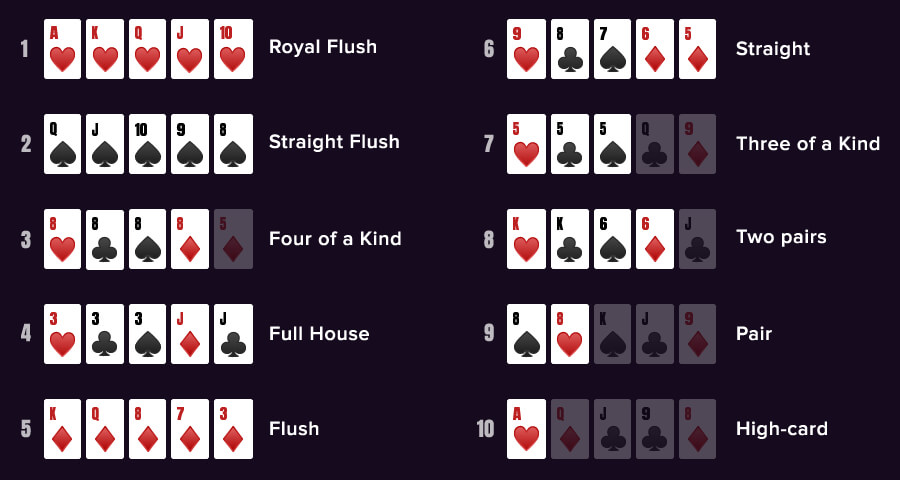
\includegraphics[width=14cm]{PokerHands}
	\caption{Lehetséges pókerkezek}
	\label{fig-pokerhands}
\end{figure}

\subsection{Használt kézkiértékelő algoritmus}

A legelterjedtebb kézkiértékelő algoritmusok azon alapulnak, hogy a kezek értékeit egy előre kiszámított kéz értékeket tároló táblából keressük ki. Ez az egyik leggyorsabb módszer, viszont a módszer egy nagy hátránya a nagy méretű tábla tárolása, amely tárhely igényes. A játékomban egy bit matematikán alapuló algoritmust használtam, aminek alapjait \acite{HandEvaluation} blog adta. Ez a módszer lassabb, mint a táblás, viszont a tárhely igényes probléma itt megszűnik.

\subsubsection{Algoritmus}

Az alábbi lépéseket kell végrehajtanunk a kézkiértékeléshez:

\begin{enumerate}
	\item Minden kártyáról el kell tárolnunk a rangját és a színét. Az inputunk 5 darab ilyen kártyából fog állni.
	\item 2 különböző bitmező létrehozása a kártyák alapján
	\begin{itemize}
		\item Az első mező a kártyák rangjának előfordulásáról tartalmaz 15~biten információt. Az egyes biteken azt fogjuk jelölni, hogy az adott rangból van-e az 5 adott kártya között (1 ha van, 0 ha nincs). \Aref{tab-bitfieldvalues1} táblázatban és \aref{tab-bitfieldvalues2} táblázatban látható 1-1 példa az elő állított bitmezőről.
		
		\begin{table}[ht!]
			\centering
			\footnotesize
			\begin{tabular}{*{15}{c}}
				0 & 1 & 1 & 1 & 1 & 1 & 0 & 0 & 0 & 0 & 0 & 0 & 0 & 0 & 0\\
				A & K & Q & J & T & 9 & 8 & 7 & 6 & 5 & 4 & 3 & 2
			\end{tabular}
			\caption{[9, 10, J, Q, K] kártyákhoz tartozó első bitmező}
			\label{tab-bitfieldvalues1}
		\end{table}
		
		\begin{table}[ht!]
			\centering
			\footnotesize
			\begin{tabular}{*{15}{c}}
				0 & 1 & 0 & 0 & 0 & 1 & 0 & 0 & 0 & 0 & 0 & 0 & 0 & 0 & 0\\
				A & K & Q & J & T & 9 & 8 & 7 & 6 & 5 & 4 & 3 & 2
			\end{tabular}
			\caption{[9, 9, 9, K, K] kártyákhoz tartozó első bitmező}
			\label{tab-bitfieldvalues2}
		\end{table}
		
		\item A második mező a rangok előfordulásának számáról tárol információt 60~biten. Minden ranghoz rendelünk 4 bitet, ahol annyit jelölünk 1-el, amennyi darabunk van az adott rangból. \Aref{tab-bitfieldcounts1} táblázatban és \aref{tab-bitfieldcounts2} táblázatban látható 1-1 példa az elő állított bitmezőről.
		
		\begin{table}[ht!]
			\centering
			\footnotesize
			\begin{tabular}{*{15}{r}}
				0000 & 0001 & 0001 & 0001 & 0001 & 0001 & 0000 & 0000 & 0000 & 0000 & 0000 & 0000 & 0000 & 0000 & 0000\\
				A & K & Q & J & T & 9 & 8 & 7 & 6 & 5 & 4 & 3 & 2
			\end{tabular}
			\caption{[9, 10, J, Q, K] kártyákhoz tartozó második bitmező}
			\label{tab-bitfieldcounts1}
		\end{table}
		
		\begin{table}[ht!]
			\centering
			\footnotesize
			\begin{tabular}{*{15}{r}}
				0000 & 0011 & 0000 & 0000 & 0000 & 0111 & 0000 & 0000 & 0000 & 0000 & 0000 & 0000 & 0000 & 0000 & 0000\\
				A & K & Q & J & T & 9 & 8 & 7 & 6 & 5 & 4 & 3 & 2
			\end{tabular}
			\caption{[9, 9, 9, K, K] kártyákhoz tartozó második bitmező}
			\label{tab-bitfieldcounts2}
		\end{table}
		
	\end{itemize}
	\item kéz értékelés a második bitmező segítségével
	\begin{itemize}
		\item A második bitmező 15-el való maradékos osztásának segítségével kitudunk értékelni 6 különböző pókerkezet. Először átszámoljuk a második bitmezőt 10-es számrendszerbe, majd utána végezzük el a 15-el való maradékos osztást. Pár példa erre:
		\begin{itemize}
			\item Póker (four of a kind): [9, 9, 9, 9, K]
			kártyákhoz tartozó második bináris mező 10-es számrendszerbe átszámolva: 4504630419521536. Ez az érték maradékosan osztva 15-el egyenlő lesz 1-el. Minden lehetséges ilyen pókerkézhez tartozó érték 1-et fog visszaadni erre az osztásra.
			\item Full (full  house): Mindig 10-et fog visszaadni az osztás eredményeképpen.
			\item Drill (three of a kind): Mindig 9-et fog visszaadni az osztás eredményeképpen.
			\item Két pár (two pairs): Mindig 7-et fog visszaadni az osztás eredményeképpen.
			\item Egy pár (one pair): Mindig 6-ot fog visszaadni az osztás eredményeképpen.
			\item Magas lap (high card): Mindig 5-öt fog visszaadni az osztás eredményeképpen.
		\end{itemize}
		
		A varázslat az, hogy mind a hat pókerkéz a fenti módszerrel történő számolás mindig ugyanazt az eredményt adja, függetlenül attól, hogy mi a tényleges öt lap. Amit a maradékos osztás 15-el csinál, az egyenértékű az egyes 4 bites kártyák értékének összegzésével. Tehát a [2, 2, 2, 3, 3] kártyák esetében ez pl. 0111 + 0011 amit binárisan összeadva, majd átszámolva 10-et kapunk. És ez mind a 6 pókerkéznél így fog működni.
	\end{itemize}
	\item sorok ellenőrzése
	\begin{itemize}
		\item A \emph{sorok} ellenőrzéséhez az első bitmezőt fogjuk felhasználni. Az első bitmezőn bitenkénti ÉS műveletet alkalmazunk önmagának negatívjával. Ennek eredményeképpen megkapjuk az LSB-t, ami a bináris szám ábrázolásának legjobb oldali bitjére utal. Majd ezután, ha elosztjuk az eredeti bitmezőt az LSB-vel, akkor megtudjuk állapítani, hogy a pókerkéz \emph{sor}-t tartalmaz-e. Ha az osztás eredménye pontosan egyenlő 11111-el, azaz decimálisan 31-el, akkor \emph{sorunk} van, ellenkező esetben pedig nincs \emph{sorunk}. Ez a módszer minden \emph{sorra} működni fog, kivéve az \emph{ász-alacsony sorra}, amit egy külön ellenőrzéssel megtudunk állapítani. Ha az első bitmezőnk pontosan egyenlő az alábbi bitmezővel: 100000000111100, akkor \emph{ász-alacsony sorunk} van.
	\end{itemize}
	\item flush ellenőrzése
	\begin{itemize}
		\item A \emph{flush} ellenőrzésénél nincs szükségünk bit matematikára, szimplán csak azt kell megnéznünk, hogy a kapott 5 input kártya közül, mindnek megegyezik a színe. Ha mindegyik ugyanolyan színű, akkor a pókerkéz \emph{flush}, ellenkező esetben pedig nem. Ha \emph{flush} kezünk van és az előző ellenőrzés szerint \emph{sorunk} is van, akkor \emph{straight flush} kezünk van. Az első bitmező segítségével pedig tudjuk ellenőrzini a \emph{royal flush}-t is. Hasonló módon mint az \emph{ász-alacsony sornál} itt is az első bitmezőt kell ellenőriznünk. Ha az első bitmezőnk pontosan egyenlő az alábbi bitmezővel: 111110000000000, akkor \emph{royal flush} pókerkezünk van.
	\end{itemize}
	\item döntetlenek eldöntése
	\begin{itemize}
		\item Abban az esetben, ha két pókerkéz azonos típusú, a döntetleneket úgy döntjük el, hogy az 5 kártyát először az előfordulás sorrendje, majd a rangja szerint rendezzük, és bitek eltolásával összehasonlítható pontszámot hozunk létre az alábbiak szerint:
		\begin{itemize}
			\item Az első kártya értékét kettes számrendszerben eltoljuk balra 16-al
			\item A második kártya értékét kettes számrendszerben eltoljuk balra 12-vel
			\item A harmadik kártya értékét kettes számrendszerben eltoljuk balra 8-cel
			\item A negyedik kártya értékét kettes számrendszerben eltoljuk balra 4-el
			\item Az ötödik kártya értékét nem toljuk el
		\end{itemize}  
		Ezután kombináljuk mind az öt létrejött számot bitenkénti VAGY művelettel és ennek az eredménye lesz a döntetleneket eldöntő pontszáma a pókerkéznek, ahol minél magasabb ez a pontszám, annál jobb kezünk van.
	\end{itemize}
	
\end{enumerate}

A teljes algoritmus tehát röviden így működik:

\begin{enumerate}
	\item Eltároljuk az 5 kártyánkról a szükséges szín és rang adatokat.
	\item A második bitmezőn maradékos osztást használva ellenőrizzük, hogy póker, full, drill, két pár, egy pár vagy magas lap pókerkezünk van-e.
	\item Az első bitmező LSB-vel történő osztásával ellenőrizzük a sorokat, majd elvégezzük az ász-alacsony sorok extra ellenőrzését.
	\item Ellenőrizzük, hogy van-e öt azonos színű lap a flush-höz, beleértve a royal flush extra ellenőrzését is.
	\item A döntetleneket felbontjuk a pókerkezekhez kiszámolt bizonyos pontszámok összehasonlításával.
\end{enumerate}

\section{Többjátékos kapcsolat megvalósítása}

\subsection{Kapcsolat kezelése a PC oldalon}
\subsection{Kapcsolat kezelése a Mobile oldalon}

\section{Játékmenet megvalósítása}

\subsection{Modul1}
\subsection{Modul2}

\chapter{Tesztelés}

\section{SharedDLL tesztelése}
\section{PC játék tesztelése}
\section{Mobile játék tesztelése}
\section{Általános tesztelés}

\chapter*{Összegzés}
\addcontentsline{toc}{chapter}{Összegzés}

\begin{thebibliography}{2}
	\addcontentsline{toc}{chapter}{\bibname}
	\bibitem{WikipediaGameEngine}
	\textsc{Wikipedia}: \emph{Game engine}, Wikipedia, az online enciklopédia, elérhető: \url{https://en.wikipedia.org/wiki/Game_engine} [Letöltve: 2025-02-28]
	\bibitem{WikipedaiUnreal}
	\textsc{Wikipedia}: \emph{Unreal Engine}, Wikipedia, az online enciklopédia, elérhető: \url{https://en.wikipedia.org/wiki/Unreal_Engine} [Letöltve: 2025-02-28]
	\bibitem{GitHubGodot}
	\textsc{GitHub}: \emph{Godot}: \url{https://github.com/godotengine/godot)} [Letöltve: 2025-02-28]
	\bibitem{WikipediaUnity}
	\textsc{Wikipedia}: \emph{Unity (game engine)}, Wikipedia, az online enciklopédia, elérhető: \url{https://en.wikipedia.org/wiki/Unity_(game_engine)} [Letöltve: 2025-02-28]
	\bibitem{MediumMultiplayer}
	\textsc{Jamal Aladdin}: \emph{The Evolution of Multiplayer Gaming: A Journey Through Time}, Jamal Aladdin blogja, elérhető:
	\url{https://medium.com/@Jamal_Aladdin/the-evolution-of-multiplayer-gaming-a-journey-through-time-e34ef59294c2} [Letöltve: 2025-02-28]
	\bibitem{MediumClientServer}
	\textsc{Lem Apperson}: \emph{Beginning Game Development: Client-Server Architecture}, Lem Apperson blogja, elérhető:
	\url{https://medium.com/@lemapp09/beginning-game-development-client-server-architecture-1b7676d80dea} [Letöltve: 2025-02-28]
	\bibitem{WikipediaP2P}
	\textsc{Wikipedia}: \emph{Peer-to-peer}, Wikipedia, az online enciklopédia, elérhető: \url{https://hu.wikipedia.org/wiki/Peer-to-peer} [Letöltve: 2025-03-02]
	\bibitem{MediumP2P}
	\textsc{Tashi Protocol}: \emph{Peer-to-Peer Gaming}, Tashi Protocol blogja, elérhető:
	\url{https://medium.com/tashi-gg/peer-to-peer-gaming-9991600c6707} [Letöltve: 2025-03-02]
	\bibitem{WikipediaPoker}
	\textsc{Wikipedia}: \emph{Póker}, Wikipedia, az online enciklopédia, elérhető: \url{https://hu.wikipedia.org/wiki/P%C3%B3ker} [Letöltve: 2024-11-12]
	\bibitem{WikipediaTexasholdem}
	\textsc{Wikipedia}: \emph{Texas Hold'Em}, Wikipedia, az online enciklopédia, elérhető: \url{https://hu.wikipedia.org/wiki/Texas_Hold%E2%80%99Em} [Letöltve: 2024-11-13]
	\bibitem{HandEvaluation}
	\textsc{Jonathan Hsiao}: \emph{Evaluating Poker Hands with Bit Math}, Jonathan Hsiao blogja, elérhető: \url{https://jonathanhsiao.com/blog/evaluating-poker-hands-with-bit-math} [Letöltve: 2025-02-25]
	\bibitem{Szurdi}
	\textsc{Szurdi András}: \emph{Pókerkönyv. Kezdőknek és haladóknak}, Ciceró, Budapest, 1995.
	\bibitem{Varga}
	\textsc{Varga Ervin}: \emph{Póker alapkönyv}, Vagabund, Kecskemét, 2008.
\end{thebibliography}

% Aláírt, szkennelt nyilatkozat beillesztése a szakdolgozat végére
%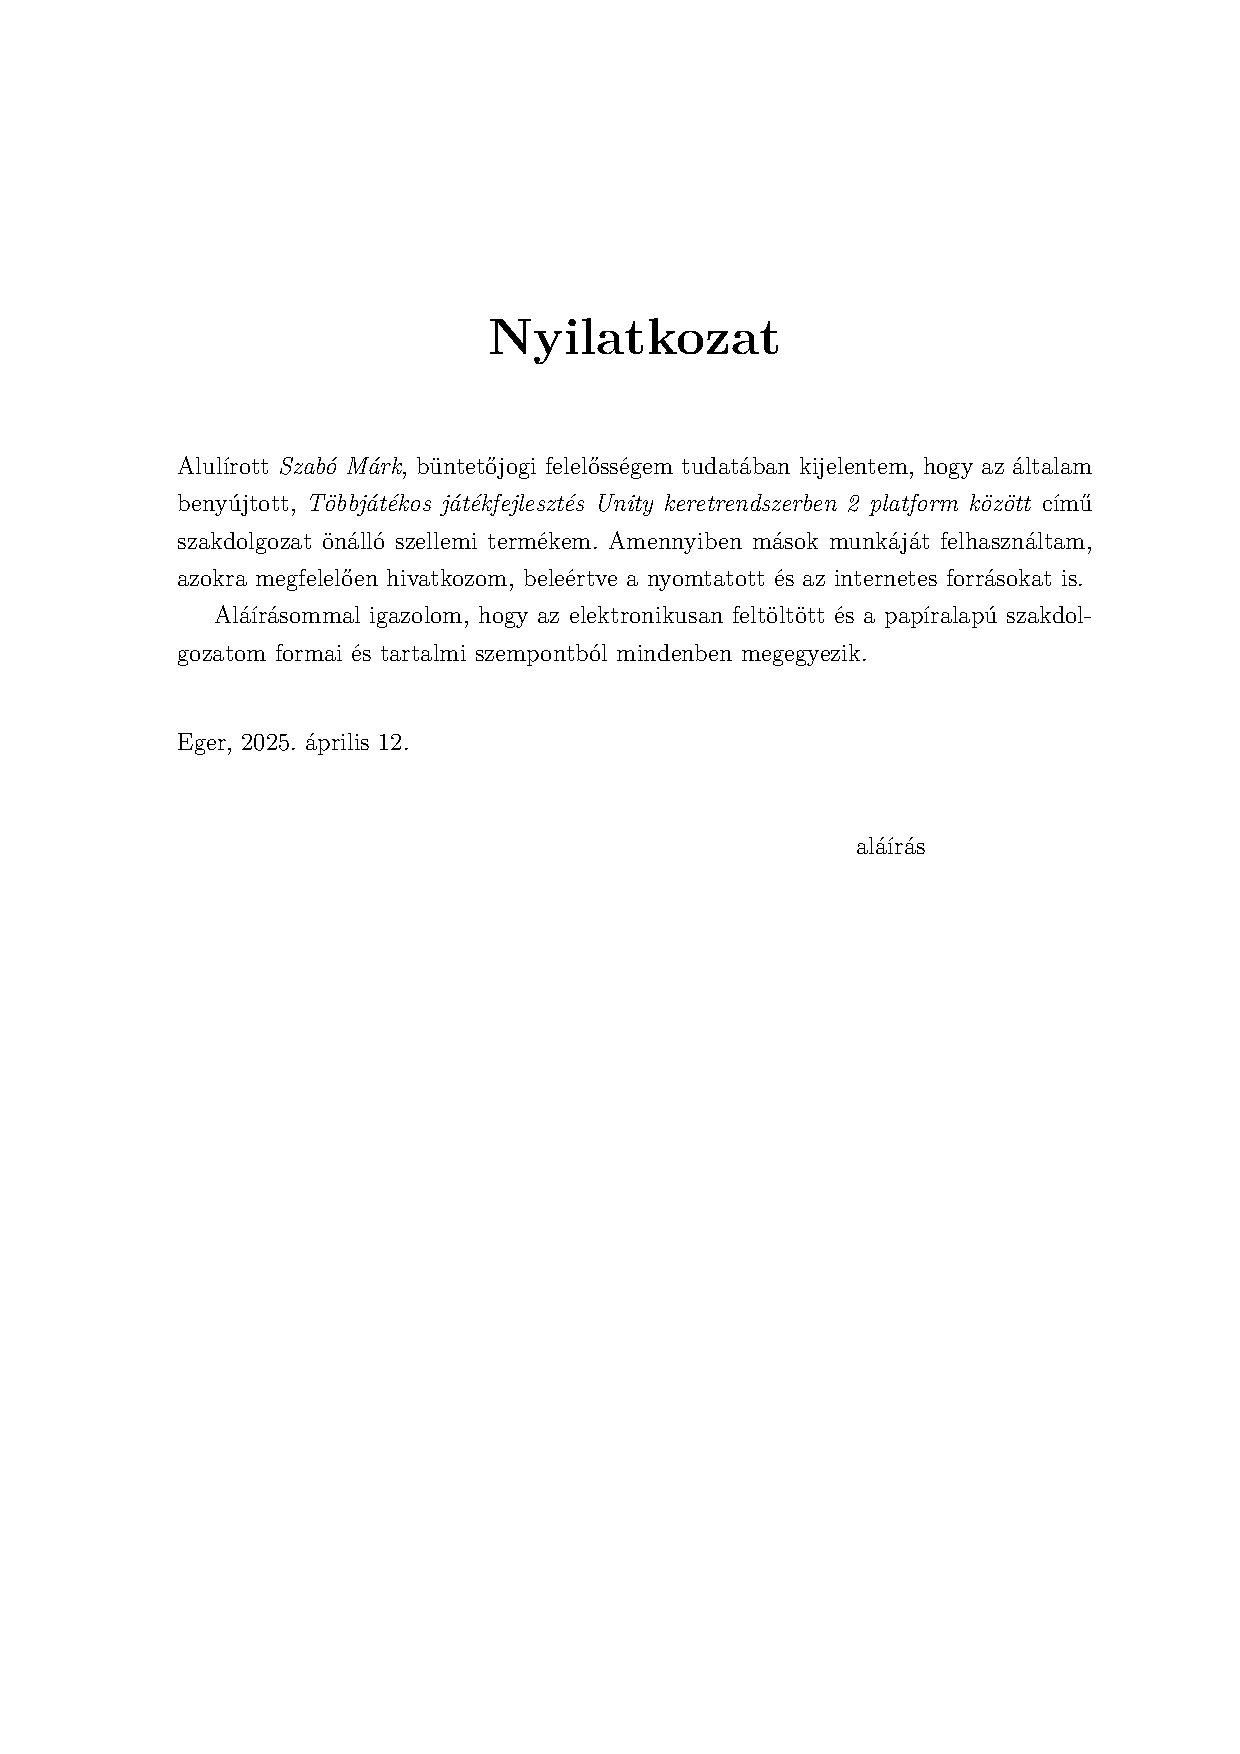
\includepdf{nyilatkozat/nyilatkozat.pdf}
\end{document}